\documentclass[tikz,border=5pt]{standalone}
\usepackage{tikz}
\usetikzlibrary{shapes,arrows,positioning}

\begin{document}
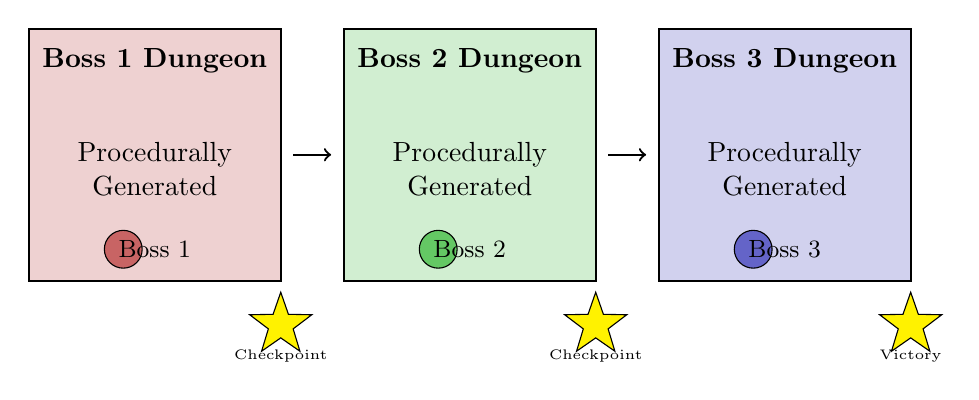
\begin{tikzpicture}[scale=0.8]
    % Define colors for different boss sections
    \definecolor{boss1}{RGB}{200,100,100}
    \definecolor{boss2}{RGB}{100,200,100}
    \definecolor{boss3}{RGB}{100,100,200}

    % Boss 1 Section (Red theme)
    \draw[fill=boss1!30, thick] (0,0) rectangle (4,4);
    \node at (2,3.5) {\textbf{Boss 1 Dungeon}};
    \node at (2,2) {Procedurally};
    \node at (2,1.5) {Generated};
    \draw[fill=boss1] (1.5,0.5) circle (0.3);
    \node at (2,0.5) {\small Boss 1};

    % Arrow
    \draw[->,thick] (4.2,2) -- (4.8,2);

    % Boss 2 Section (Green theme)
    \draw[fill=boss2!30, thick] (5,0) rectangle (9,4);
    \node at (7,3.5) {\textbf{Boss 2 Dungeon}};
    \node at (7,2) {Procedurally};
    \node at (7,1.5) {Generated};
    \draw[fill=boss2] (6.5,0.5) circle (0.3);
    \node at (7,0.5) {\small Boss 2};

    % Arrow
    \draw[->,thick] (9.2,2) -- (9.8,2);

    % Boss 3 Section (Blue theme)
    \draw[fill=boss3!30, thick] (10,0) rectangle (14,4);
    \node at (12,3.5) {\textbf{Boss 3 Dungeon}};
    \node at (12,2) {Procedurally};
    \node at (12,1.5) {Generated};
    \draw[fill=boss3] (11.5,0.5) circle (0.3);
    \node at (12,0.5) {\small Boss 3};

    % Checkpoint markers
    \node[star, star points=5, star point ratio=2.5, fill=yellow, draw=black] at (4,-0.7) {};
    \node at (4,-1.2) {\tiny Checkpoint};

    \node[star, star points=5, star point ratio=2.5, fill=yellow, draw=black] at (9,-0.7) {};
    \node at (9,-1.2) {\tiny Checkpoint};

    \node[star, star points=5, star point ratio=2.5, fill=yellow, draw=black] at (14,-0.7) {};
    \node at (14,-1.2) {\tiny Victory};

\end{tikzpicture}
\end{document}
